\documentclass[11pt]{article}
\usepackage[left=3.5cm,right=3.5cm,top=2.5cm,bottom=2.5cm]{geometry}
%\usepackage[spanish]{babel}

\usepackage{amsmath,amsfonts,amsthm}
\usepackage{enumitem,mathtools,graphicx}
\setenumerate[0]{label=(\alph*)}

\newtheorem{definition}{Definición}
\newtheorem{exercise}{Ejercicio}
\newtheorem*{sol}{Solución}

\newcommand\N{\mathbb N}
\newcommand\R{\mathbb R}

\title{Análisis numérico para ecuaciones diferenciales \\
Tarea 1 - Introducción a los métodos de un paso}
\author{Jorge Alfredo Álvarez Contreras}

\begin{document}
\maketitle

\begin{definition}[Método de Euler]
  Dado un problema de valores iniciales
  \begin{equation}\label{eq:pvi}
    \left\{
      \begin{aligned}
        y'(t) &= f(t,y) \\
        y(0) &= y_0
      \end{aligned}
    \right.
  \end{equation}
\end{definition}

\begin{exercise}
  Demuestre que el método de Euler es cero-estable cuando es aplicado
  al problema de valores iniciales $y'=-1/y^{2}$, $y(0)=y_0$, donde
  $y_0\in[a,b]$ para $0<a<b$.
\end{exercise}

\begin{sol}
  La situación del problema está dada por el PVI \eqref{eq:pvi},
  donde $f(t,y)=f(y)=-\frac{1}{y^{2}}$.
  Fíjese $N\geq 1$ tan grande como se quiera,
  de modo que, al menos, $a\geq 1 / N$. Entonces $f=f(y)$ es de
  Lipschitz en $[1 / N,\infty)$, ya que para $y_1,y_2\geq 1 / N$ se
  tiene $N\geq \frac{1}{y_1}$ y $N\geq \frac{1}{y_2}$, de modo que
  \begin{align}
    |f(y_2)-f(y_1)|
    &= \left|-\frac{1}{y_2^{2}}+\frac{1}{y_1^{2}}\right| \\
    &= \left|\frac{y_2^{2}-y_1^{2}}{y_1^{2}y_2^{2}}\right| \\
    &= \frac{y_2+y_1}{y_1^{2}y_2^{2}} |y_2-y_1| \\
    &=
    \left(
      \frac{1}{y_1^{2}y_2}
      +
      \frac{1}{y_1y_2^{2}} 
    \right)
    |y_2-y_1| \\
    &\leq 2N^{3} |y_2-y_1|
  .\end{align}

  Por el teorema de estabilidad cero, esto implica que, para
  intervalos de tiempo $[0,T]$ pequeños (lo suficientemente pequeños
  como para que $y(t)$ no disminuya por debajo de $1 / N$)
  entonces el método de Euler es cero-estable.
\end{sol}

\begin{exercise}
  Implemente en Python los métodos de Euler y Heun. Posteriormente
  utilice estos métodos para resolver el PVI
  \begin{equation}
    \left\{
      \begin{aligned}
        y' &= yt^{3} - 3y / 2, \\
        y(0) &= 1,
      \end{aligned}
    \right.
  \end{equation}
  con $h=0.2$ en $t\in [0,2]$. Elabore dos gráficas, una con la
  aproximación obtenida contra la solución analítica y otra del error
  puntual.
\end{exercise}
\begin{sol}
  \begin{figure}[ht]
    \centering
    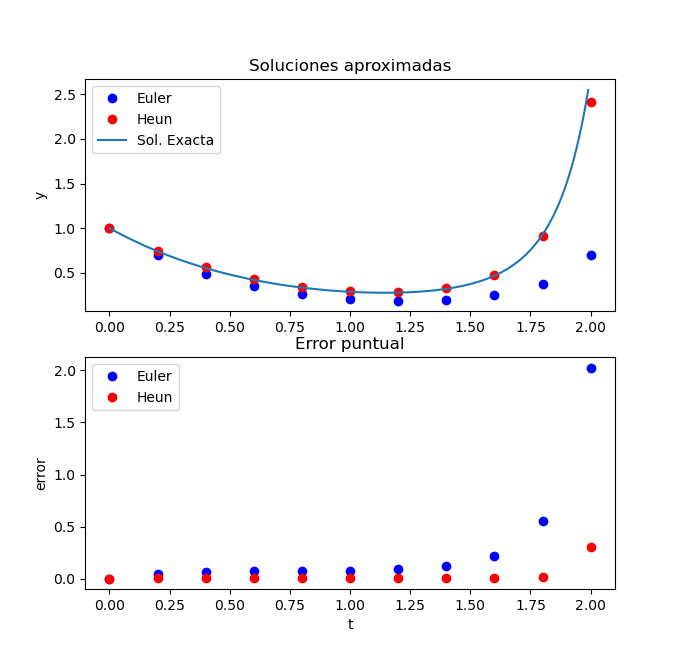
\includegraphics[width=0.5\textwidth]{img/jaac_tarea1_ejercicio2}
    \caption{Resultados del ejercicio 2: soluciones aproximadas para
      $y'(t)=yt^{3}-\frac{3y}{2}$.
      La solución exacta es $y(t)=\exp(t^{4} / 4 - 3t / 2)$.}
    \label{fig:exe_1}
  \end{figure}
\end{sol}

\begin{exercise}
  Adapte los programas de Python que elaboró en el ejercicio anterior
  para resolver sistemas de ecuaciones. Utilice dichos programas para
  resolver numéricamente el oscilador de Van der Pol:
  \begin{equation}
    y'' + (y^{2}-1)y' + y = 0
  .\end{equation}
  Grafique las órbitas con $y(0)=0$, $y'(0)=1$ y con $y(0)=-2$,
  $y'(0)=3$. Utilice el mismo valor de $h$ para ambos métodos y
  presente dichas órbitas en una figura distinta para cada método.
\end{exercise}
\begin{sol}
  \leavevmode
  \begin{figure}[hb]
    \centering
    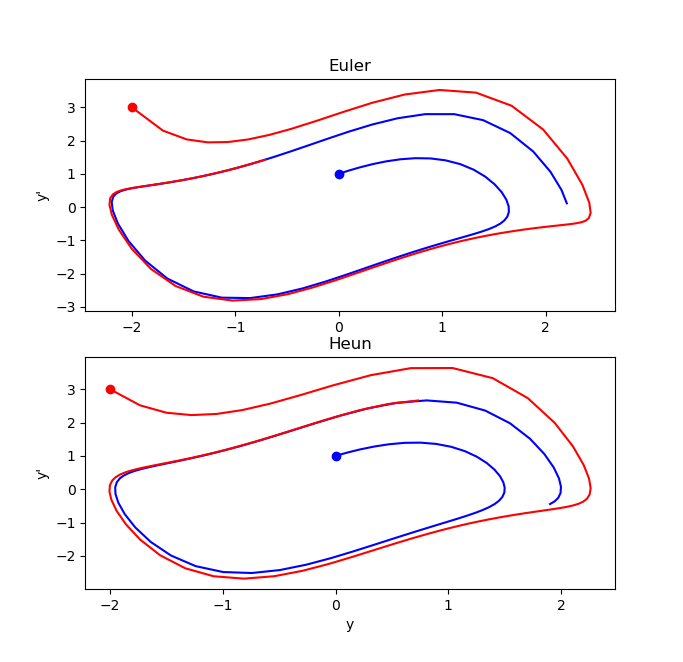
\includegraphics[width=0.5\textwidth]{img/jaac_tarea1_ejercicio3}
    \caption{Resultados del ejercicio 3: soluciones aproximadas para
      el oscilador de Van der Pol: $y'' + (y^{2}-1)y' + y = 0$}
    \label{fig:exe_2}
  \end{figure}
\end{sol}

\begin{exercise}
  Calcule el error de truncamiento local y el orden del método
  trapezoidal.
\end{exercise}
\begin{sol}
  El método trapezoidal está definido como
  \begin{equation}
    u_{n+1} = u_n + \frac{h}{2}[f_n + f_{n+1}]
  \end{equation}
  con $u_0=y_0$.
  El error de truncamiento local $\tau_{n+1}$ es el cociente
  $\epsilon_{n+1} / h$, donde
  \begin{equation}
    y_{n+1} = y_n + \frac{h}{2}[f(t_n,y_n)+f(t_{n+1},y_{n+1})] +
    \epsilon_{n+1}
  .\end{equation}
  Expandiendo en serie de Taylor:
  \begin{equation}\label{eq:taylor_trapezoidal}
    \begin{split}
    &\hspace{-5mm}
    y_{n}+hy'_n+\frac{h^{2}}{2}y''_n+\frac{h^{3}}{3!}y'''(\xi)
    \\
    &=
    y_n
    +
    \frac{h}{2} \left[
      2y'_n + h Df(t_n,y_n)((1,y'_n))
      + \frac{h^{2}}{2} D^{2}f(z)((1,y'_n),(1,y'_n))
    \right]
    + \epsilon_{n+1},
    \end{split}
  \end{equation}
  donde $\xi\in(t_n,t_{n+1})$ y $z\in\R^{2}$ es un vector en el
  segmento que conecta a los puntos $(t_n,y_n)$ y $(t_{n+1},y_{n+1})$.
  Notando que
  \begin{align}
    Df(t_n,y_n)((1,y'_n))
    &= \frac{\partial f}{\partial t}(t_n,y_n)
    + \frac{\partial f}{\partial y}(t_n,y_n)y'_n \\
    &= y''_n
  \end{align}
  la expresión \eqref{eq:taylor_trapezoidal} se simplifica a
  \begin{equation}
    \frac{h^{3}}{3!}y'''(\xi)
    =
    \frac{h^{3}}{4} D^{2}f(z)((1,y'_n),(1,y'_n))
    + \epsilon_{n+1},
  .\end{equation}
  Luego,
  \begin{equation}
    \tau_{n+1}(h)
    =
    \frac{\epsilon_{n+1}}{h}
    =
    \frac{h^{2}}{2}
    \left(
      \frac{1}{3}y'''(\xi)
      -
      \frac{1}{2}D^{2}f(z)((1,y'_n),(1,y'_n))
    \right)
    = O(h^{2})
  .\end{equation}
  
\end{sol}

\begin{exercise}
  Considere el método
  \begin{equation}
    u_{n+1} = u_n + h[af_n + bf(t_n+\alpha h,u_n+\beta h f_n)]
  \end{equation}
  donde $a,b,\alpha,\beta$ son parámetros reales.
  \begin{enumerate}
    \item
      Establezca condiciones sobre los parámetros $a,b,\alpha,\beta$ 
      para garantizar que el método es de primer orden.
    \item
      Pruebe que existe una combinación de estos parámetros tal que el
      método es de segundo orden. ¿Existe alguna combinación de las
      constantes de tal manera que el orden es mayor a $2$?
  \end{enumerate}
\end{exercise}

\begin{exercise}
  Considere el método de un paso dado por
  \begin{equation}
    u_{n+1} = u_n + h \left[
      f_n + \frac{h}{2}g \left(
        t_n + \frac{1}{3}h,
        u_n + \frac{1}{3}hf_n
      \right)
    \right]
  ,\end{equation}
  donde $g=f_t+ff_y$. Muestre que el método es de orden $3$.
\end{exercise}

\begin{exercise}
  Demuestre el teorema de convergencia 11.2 del libro de Quarteroni:
\end{exercise}

\end{document}
